\section{Experimental Evaluation}\label{Se:experiments}

In this section, we describe the \Tool\ implementation, and present two sets of experiments that we have conducted to evaluate our approach.

\subsection{The \Tool\ System}\label{Se:impl}

\paragraph{Implementation} Similarly to existing tools like TaintDroid, \Tool\ is implemented as an instrumented version of the Android SDK. Specifically, we have instrumented version 4.1.1\_r6 of the SDK, which was chosen intentionally to match the most recent version of TaintDroid.\footnote{
	\href{http://appanalysis.org/download.html}{http://appanalysis.org/download.html}
} The experimental data we present indeed utilizes TaintDroid for tag propagation (as required for accurate resolution for relevant values).

Beyond the TaintDroid instrumentation scheme, the \Tool\ scheme specifies additional behaviors for sources and sinks within the SDK. At source points, a hook is added to record the private value read by the source statement (which acts as a reference value). At sink points, a hook is installed to apply Bayesian reasoning regarding the legitimacy of the sink.

Analogously to TaintDroid, \Tool\ performs privacy monitoring over APIs for file-system access and manipulation, inter-application and socket communication, reading the phone's state and location, and sending of text messages. \Tool\ also monitors the HTTP interface, camera, microphone, bluetooth and contacts. \OC{As explained in \secref{pseudo}, each of the privacy sources monitored by \Tool\ is mirrored by a tag/feature. The full list of features is as follows: \emph{IMEI}, \emph{IMSI}, \emph{AndroidID}, \emph{Location}, \emph{Microphone}, \emph{Bluetooth}, \emph{Camera}, \emph{Contacts}, \emph{FileSystem}.}

The \Tool\ implementation is configurable, enabling the user to switch between distance metrics as well as enable/disable information-flow tracking for precise/heuristic determination of relevant values. (See \secref{points}.) In our experiments, we tried both the Levenshtein and the Hamming metrics, but found no observable differences, and so we report the results only once. Our reasoning for why the metrics are indistinguishable is because we apply both to equal-length strings (see \secref{similarstr}), and have made sure to apply the same metric both offline and online, and so both metrics achieve a very similar effect in the Bayesian setting.

\paragraph{Training} To instantiate \Tool\ with the required estimates, as explained in \secref{estprob}, we applied the following methodology:
%
First, to estimate $\Pr(\emph{legitimate})$, we relied on (i) an extensive study by Hornyack et al. spanning 1,100 top-popular free Android apps~\cite{HHJSW:CCS11}, as well as (ii) a similarly comprehensive study by Enck et al.~\cite{EOMC:SEC11}, which also spans a set of 1,100 free apps. According to the data presented in these studies, approximately one out of three release points is illegitimate, and thus $\hat{\Pr}(\emph{legitimate})=0.66$ and complementarily 
$\hat{\Pr}(\emph{illegitimate}) = 1-0.66 \approx 0.33$.

For the conditional probabilities $\hat{\Pr}(X_i = x_{ij} | Y=y_k)$,  we queried Google Play for the 100 most popular apps (across all domains) in the geography of one of the authors. We then selected at random 35 of these apps, and analyzed their information-release behavior using debug breakpoints 
(which we inserted via the {\tt adb} tool that is distributed as part of the Android SDK). 

Illegitimate leaks that we detected offline mainly involved (i) location information and (ii) device and user identifiers, which is consistent with the findings reported by past studies~\cite{HHJSW:CCS11,EOMC:SEC11}. We confirmed that illegitimate leaks are largely correlated with high similarity between private data and sink arguments, and so we fixed six distance levels for each private item: $[0,4]$ and ``$\geq 5$''. (See \secref{featext}.) Finally, to avoid from zero estimates for conditional probabilities while also minimizing data perturbation, we set the ``smoothening'' factor $l$ in \equref{smoothEstimate} at 1, where the illegitimate flows we detected were in the order of several dozens per private item. 

\subsection{Experimental Hypotheses}

%We conducted all of our experiments on clean virtual-machine images with 4GB of RAM running version 12.04.2 LTS of the Ubuntu Linux distribution. For our experiments, we used the Android mobile device emulator included with the Android SDK. We loaded the TaintDroid and \Tool\ images into separate emulators running on different clones of the virtual machine. For TaintDroid, we followed the installation and setup steps provided online.

In our experimental evaluation of \Tool, we tested two hypotheses:
\begin{compactenum}
	\item \underline{H1: Accuracy.} Bayesian reasoning about the legitimacy of information release, as implemented in \Tool, yields a significant improvement in accuracy compared to the baseline of 
	information-flow tracking.
	\item \underline{H2: Power of Bayesian Analysis.} \Tool\ remains effective under relaxation of the tag-based method for detection of relevant values, and its stability and applicability to real-world applications improve.
\end{compactenum}

\subsection{H1: Accuracy of \Tool}\label{Se:overhead}

For accuracy measurement, we applied both TaintDroid and \Tool\ to DroidBench, an independent and publicly available collection of benchmarks serving as testing ground for both static and dynamic privacy enforcement algorithms. DroidBench models a large set of realistic challenges in leakage detection, including precise tracking of sensitive data through containers, handling of callbacks, field and object sensitivity, lifecycle modeling, inter-app communication, reflection and implicit flows. The DroidBench suite consists of 50 cases.

The results we obtained for both TaintDroid and \Tool\ on version 1.1 of DroidBench are summarized in \tableref{accuracyDBench}. The findings reported by \Tool\ are publicly available.\footnote{
	See archive file droidbench.zip at \href{https://www.dropbox.com/sh/ggrcvqsbkiubmlb/faSUXmr9xK}{https://www.dropbox.com/sh/ggrcvqsbkiubmlb/faSUXmr9xK}.
} We excluded from the table (i) 8 benchmarks that crash at startup, as well as (ii) 5 benchmarks that leak data via callbacks that we did not manage to trigger (e.g., {\tt onLowMemory()}), for a total of 37 benchmarks. For both of these categories, both TaintDroid and \Tool\ were naturally unable to detect leakages.

Overall, TaintDroid detects 31 true leakages while also reporting 17 false positives, whereas our approach suffers from 2 false negatives, discovering 30 of the true leakages while flagging only 1 false positive. We summarize the results as (i) the average across all app scores, shown outside the parentheses (0.96 for \Tool\ vs 0.69 for TaintDroid), as well as (ii) the global accuracy score, computed as TPs / (TPs + FPs + Fns) (0.91 vs 0.65).

\begin{table*}
\begin{small}
\begin{center}
	\begin{tabular}{l|c|c|c|c|c|c|c|c}
	\multicolumn{1}{c|}{\multirow{2}{*}{Benchmark}} & \multicolumn{4}{c|}{\Tool} & \multicolumn{4}{c}{TaintDroid} \\
	\cline{2-9} 
	& TPs & FPs & FNs & accuracy & TPs & FPs & FNs & accuracy \\	
	\hline
	{\tt ActivityCommunication1} 	& 1 & 0 & 0 & 1.0 & 1 & 0 & 0 & 1.0 \\
	{\tt ActivityLifecycle1} 				& 1 & 0 & 0 & 1.0 & 1 & 0 & 0 & 1.0 \\
	{\tt ActivityLifecycle2} 				& 1 & 0 & 0 & 1.0 & 1 & 0 & 0 & 1.0 \\
	{\tt ActivityLifecycle4} 				& 1 & 0 & 0 & 1.0 & 1 & 0 & 0 & 1.0 \\
	{\tt Library2} 								& 1 & 0 & 0 & 1.0 & 1 & 0 & 0 & 1.0 \\
	{\tt Obfuscation1} 						& 1 & 0 & 0 & 1.0 & 1 & 0 & 0 & 1.0 \\
	{\tt PrivateDataLeak3} 				& 1 & 1 & 0 & 0.5 & 1 & 1 & 0 & 0.5 \\
	{\tt AnonymousClass1} 				& 0 & 0 & 0 & 1.0 & 0 & 1 & 0 & 1.0 \\
	{\tt ArrayAccess1} 						& 0 & 0 & 0 & 1.0 & 0 & 1 & 0 & 0.0 \\
	{\tt ArrayAccess2} 						& 0 & 0 & 0 & 1.0 & 0 & 1 & 0 & 0.0 \\
	{\tt HashMapAccess1} 				& 0 & 0 & 0 & 1.0 & 0 & 1 & 0 & 0.0 \\
	{\tt Button1} 								& 1 & 0 & 0 & 1.0 & 1 & 0 & 0 & 1.0 \\
	{\tt Button3} 								& 2 & 0 & 0 & 1.0 & 2 & 0 & 0 & 1.0 \\
	{\tt Ordering1} 							& 0 & 0 & 0 & 1.0 & 0 & 2 & 0 & 0.0 \\
	{\tt RegisterGlobal1} 					& 1 & 0 & 0 & 1.0 & 1 & 0 & 0 & 1.0 \\
	{\tt DirectLeak1} 						& 1 & 0 & 0 & 1.0 & 1 & 0 & 0 & 1.0 \\
	{\tt FieldSensitivity2} 					& 0 & 0 & 0 & 1.0 & 0 & 1 & 0 & 0.0 \\
	{\tt FieldSensitivity3} 					& 1 & 0 & 0 & 1.0 & 1 & 0 & 0 & 1.0 \\
	{\tt FieldSensitivity4} 					& 0 & 0 & 0 & 1.0 & 0 & 1 & 0 & 0.0 \\
	{\tt ImplicitFlow1} 						& 0 & 0 & 2 & 0.0 & 2 & 0 & 0 & 1.0 \\
	{\tt InheritedObjects1} 				& 1 & 0 & 0 & 1.0 & 1 & 0 & 0 & 1.0 \\
	{\tt ListAccess1} 						& 0 & 0 & 0 & 1.0 & 0 & 1 & 0 & 0.0 \\
	{\tt LocationLeak1} 					& 0 & 0 & 0 & 1.0 & 0 & 2 & 0 & 0.0 \\
	{\tt LocationLeak2} 					& 0 & 0 & 0 & 1.0 & 0 & 2 & 0 & 0.0 \\
	{\tt Loop1} 									& 1 & 0 & 0 & 1.0 & 1 & 0 & 0 & 1.0 \\
	{\tt Loop2} 									& 1 & 0 & 0 & 1.0 & 1 & 0 & 0 & 1.0 \\
	{\tt ApplicationLifecycle1} 			& 1 & 0 & 0 & 1.0 & 1 & 0 & 0 & 1.0 \\
	{\tt ApplicationLifecycle3} 			& 1 & 0 & 0 & 1.0 & 1 & 0 & 0 & 1.0 \\
	{\tt MethodOverride1} 				& 1 & 0 & 0 & 1.0 & 1 & 0 & 0 & 1.0 \\
	{\tt ObjectSensitivity1} 				& 0 & 0 & 0 & 1.0 & 0 & 1 & 0 & 0.0 \\
	{\tt ObjectSensitivity2} 				& 0 & 0 & 0 & 1.0 & 0 & 2 & 0 & 0.0 \\
	{\tt Reflection1} 							& 1 & 0 & 0 & 1.0 & 1 & 0 & 0 & 1.0 \\
	{\tt Reflection2} 							& 1 & 0 & 0 & 1.0 & 1 & 0 & 0 & 1.0 \\
	{\tt Reflection3} 							& 1 & 0 & 0 & 1.0 & 1 & 0 & 0 & 1.0 \\
	{\tt Reflection4} 							& 1 & 0 & 0 & 1.0 & 1 & 0 & 0 & 1.0 \\
	{\tt SourceCodeSpecific1} 		& 5 & 0 & 0 & 1.0 & 5 & 0 & 0 & 1.0 \\
	{\tt StaticInitialization1} 				& 1 & 0 & 0 & 1.0 & 1 & 0 & 0 & 1.0 \\
	\hline \hline
	{\bf total:}	& 29 & 1 & 2 & 0.96 (0.91) & 31 & 17 & 0 & 0.69 (0.65)
	\end{tabular}
	\end{center}
	\caption{\label{Ta:accuracyDBench}\Tool\ and TaintDroid findings on DroidBench}
\end{small}
\end{table*}

The results mark \Tool\ as visibly more accurate than TaintDroid with respective accuracy scores of 0.96 vs 0.69, \OC{which confirms H1}. Analysis of the per-benchmark findings reveals the following: First, the 2 false negatives of 
\Tool\ on {\tt ImplicitFlow1} are both due to proprietary (i.e., non-standard) data transformations, which are outside the current scope of \Tool. An illustrative fragment from the {\tt ImplicitFlow1} code is shown in \figref{dataTransform}. The {\tt obfuscateIMEI($\ldots$)} transformation maps IMEI digits to English letters, which is a non-standard behavior that is unlikely to arise in an authentic app.

The true positive reported by \Tool, in common with TaintDroid, is on release of sensitive data to the file system, albeit using the {\tt MODE\_PRIVATE} flag, which does not constitute a leakage problem in itself. This can be resolved by performing Bayesian reasoning not only over argument values, but also over properties of the sink API (in this case, the storage location mapped to a file handle). We intend to implement this enhancement. 

\begin{figure}
\begin{lstlisting}
TelephonyManager tm = 
    getSystemService(TELEPHONY_SERVICE);
String imei = tm.getDeviceId(); //source
String obfuscatedIMEI = obfuscateIMEI(imei); ...;
Log.i(imei); // sink

private String obfuscateIMEI(String imei) {
  String result = "";
  for (char c : imei.toCharArray()) { 
    switch(c) { 
      case '0': result += {\color{purple} 'a'}; break;
      case '1': result += {\color{purple} 'b'}; break;
      case '2': result += {\color{purple} 'c'}; break; 
      ...; } }
\end{lstlisting}
\caption{\label{Fi:dataTransform} Fragment from the DroidBench {\tt ImplicitFlow1} benchmark, which applies a proprietary transformation to private data}
\end{figure}


Beyond the false alarm in common with \Tool, TaintDroid has multiple other sources of imprecision. The main reasons for its false positives are
\begin{compactitem}
	\item coarse modeling of containers, mapping their entire contents to a single taint bit, which accounts e.g. for the false alarms on {\tt ArrayAccess\{1,2\}} and {\tt HashMapAccess1};
	\item field and object insensitivity, resulting in false alarms on {\tt FieldSensitivity\{2,4\}} and {\tt ObjectSensitivity\{1,2\}}; and more fundamentally,
	\item ignoring of data values, which causes TaintDroid to issue false warnings on {\tt LocationLeak\{1,2\}} even when location reads fail, yielding a {\tt Location} object without any meaningful information.
\end{compactitem} 
The fundamental reason for these imprecisions is to constrain the overhead of TaintDroid, such that it can meet the performance demands of online privacy enforcement. \Tool\ is able to accommodate such optimizations while still ensuring high accuracy. 

\subsection{H2: Power of Bayesian Analysis}\label{Se:practical}

The second aspect of the evaluation compared between two versions of \Tool, whose sole difference lies in the method used for detecting relevant values: In one configuration (T-BD), relevant values are detected via tag propagation. The other configuration (H-BD) uses the heuristic detailed in \secref{points} of treating all values reachable from sink arguments \OC{(either directly or via the heap graph)} up to a depth bound of $k$ as relevant, which places more responsibility on Bayesian reasoning. We set $k$ at 3 based on manual review of the data structures flowing into privacy sinks. In summary, H-BD trades accuracy for overhead reduction. H2 asserts that the tradeoff posed by H-BD is effective. 

\OC{\paragraph{Overhead} First, to quantify overhead reduction, we designed a parametric benchmark application, which consists of a simple loop that flows the device IMEI into a log file. Loop iterations perform intermediate data propagation steps. We then performed a series of experiments --- over the range of 1 to 19 propagation steps --- to quantify the relative overhead of tag propagation versus Bayesian analysis. 

The results, presented in \figref{overhead}, suggest that tag propagation is more dominant than Bayesian analysis in overall overhead 
(with a ratio of roughly 2:1), even when the set of relevant values is naively over approximated. Discussion of the methodology underlying this experiment is provided in \appendixref{methodology}.}

\begin{figure}
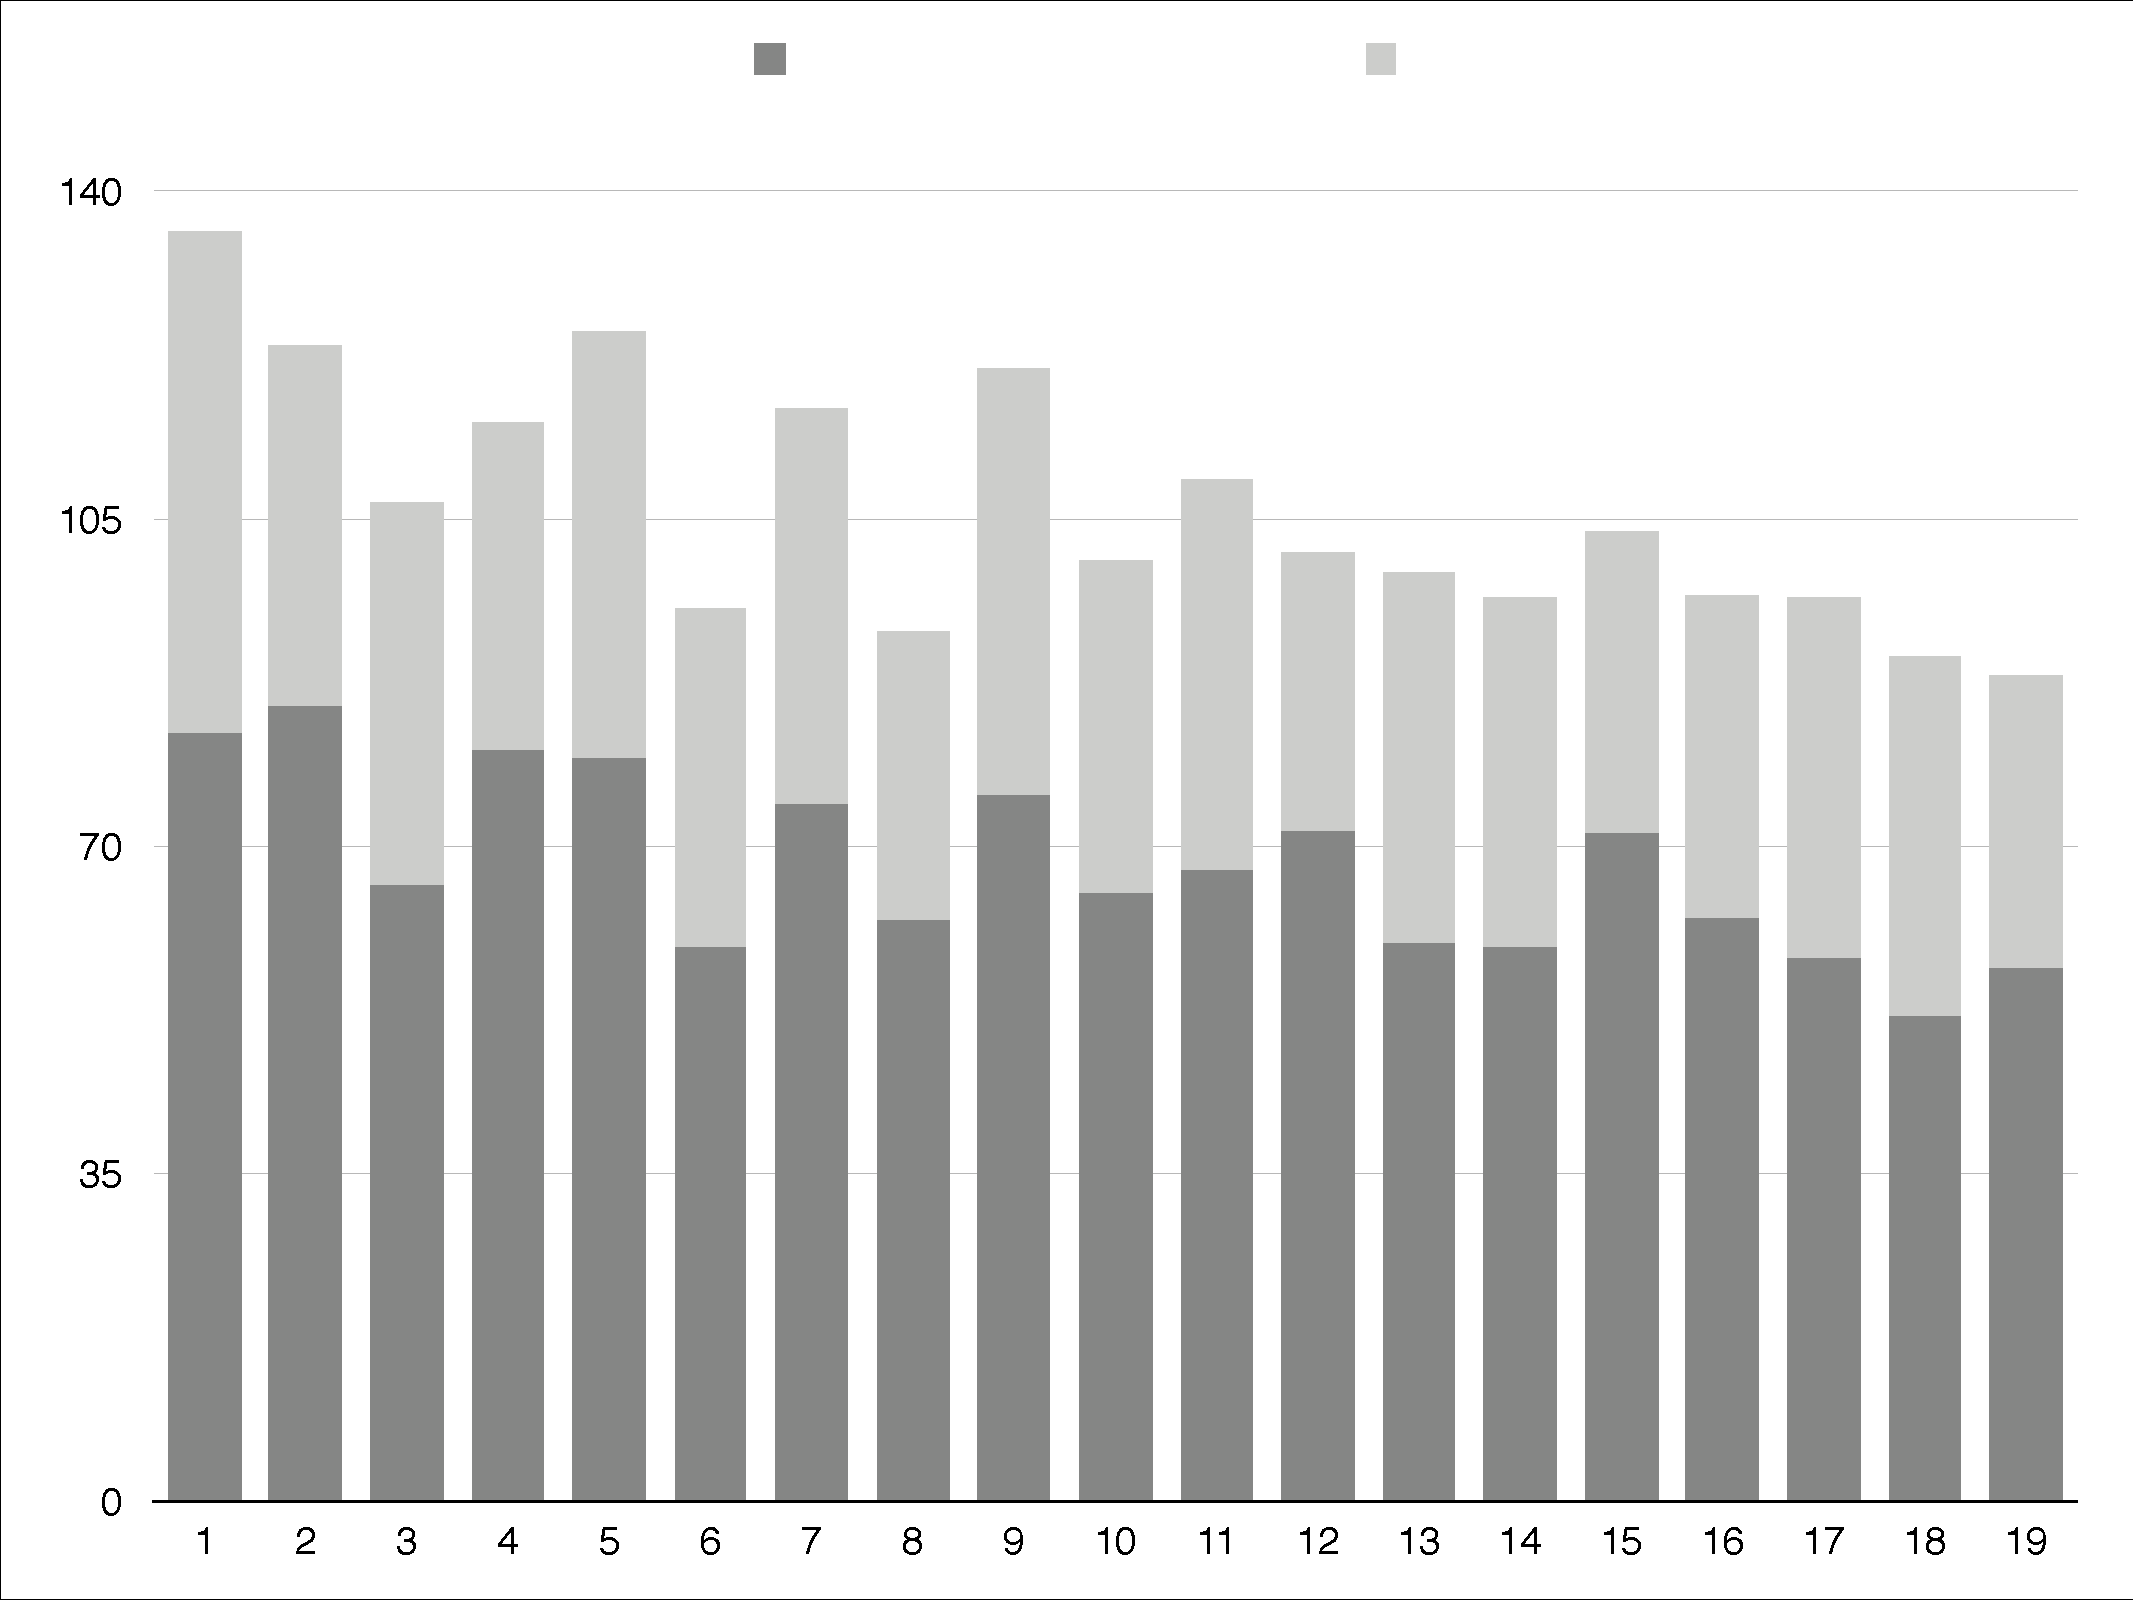
\includegraphics[width=\columnwidth]{OverheadDiagram.pdf}
\caption{\label{Fi:overhead}Overhead breakdown into tag propagation (dark grey) and Bayesian analysis at sink (pale grey), where horizontal (X) axis denotes the number of propagation steps and vertical (Y) axis denotes overhead}
\end{figure}

\OC{\paragraph{Accuracy} For accuracy comparison, we considered real-world benchmark applications.} These are listed in the first two columns of \tableref{realworld}. To select the apps, ensuring no biases, we applied the following methodology: We started from the 65 Google Play apps not chosen for the training phase. We then excluded 8 apps that do not have permission to access sensitive data and/or perform release operations (i.e., their manifest does not declare sufficient permissions out of {\tt INTERNET}, {\tt READ\_PHONE\_STATE}, {\tt SEND\_SMS}, etc), as well as 3 apps that we did not manage to install properly, resulting in 54 apps that installed successfully and exercise privacy sources and sinks.
 
We deployed the apps under the two \Tool\ configurations. Each execution was done from a clean starting state. 
The third column of \tableref{realworld} denotes whether our exploration of the app was exhaustive. By that we mean exercising all the UI points exposed by the app in a sensible order. Ideally we would do so for all apps. However, (i) some of the apps, and in particular gaming apps, had stability issues, and (ii) certain apps require SMS-validated sign in, which we did not perform. We did, however, create Facebook, Gmail and Dropbox accounts to log into apps that demand such information yet do not ask for SMS validation. We were also careful to execute the exact same crawling scenario under both the T-BD and H-BD configurations. We comment, from our experience, that most data leaks happen when an app launches, \OC{and initializes advertising/analytics functionality}, and so for apps for which deep crawling was not possible the results are still largely meaningful. 
 
The complete results are listed in \tableref{realworldAll}. The last eight columns of \tableref{realworld} summarize the findings by H-BD and T-BD, respectively, at the granularity of privacy items: the device number, Android and device identifiers, and location. 
%
%
The warnings reported by the H-BD configuration are available for review.\footnote{
	See archive file realworldapps.zip at \href{https://www.dropbox.com/sh/ggrcvqsbkiubmlb/faSUXmr9xK}{https://www.dropbox.com/sh/
	ggrcvqsbkiubmlb/faSUXmr9xK}.
}
%
We manually classified the findings into true positives (TPs) and false positive (FPs). For this classification, we scrutinized the reports by the two configurations, and also --- in cases of uncertainty --- decompiled and/or reran the app to examine its behavior more closely. 

\begin{figure*}
\begin{minipage}[b]{0.95\columnwidth}
\begin{lstlisting}
$\fbox{source : private value}$
    GeoCoder.getFromLocation(...) : [ Lat: ..., Long: ..., 
	    Alt: ..., Bearing: ..., ..., $\textbf{IL}$ ] 
	    
$\fbox{sink : arguments}$
  WebView.loadUrl(...) : http://linux.appwiz.com/
    profile/72/72_exitad.html?
    p1=RnVsbCtBbmRyb2lkK29uK0VtdWxhdG9y&
    p2=Y2RmMTUxMjRlYTRjN2FkNQ%3d%3d&
    ...    
    LOCATION=$\textbf{IL}$&
    ...
    MOBILE_COUNTRY_CODE=&
    NETWORK=WIFI
\end{lstlisting}
\caption{\label{Fi:ios7}Suppressed spurious leakage on {\tt ios7lockscreen}}
\end{minipage}
\hfill
\begin{minipage}[b]{0.95\columnwidth}
\begin{lstlisting}
$\fbox{source : private value}$
  Settings$\$$Secure.getString(...) : $\textbf{cdf15124ea4c7ad5}$
  
$\fbox{sink : arguments}$
  FileOutputStream.write(...) : 
    <?xml version='1.0' encoding='utf-8' 
    standalone='yes' 
    ?><map><string 
    name="openudid">$\textbf{cdf15124ea4c}$
\end{lstlisting}
\caption{\label{Fi:fruitninja}Suppressed spurious leakage on {\tt fruitninjafree}}
\end{minipage}
\end{figure*}

%For \Tool\ we report two numbers: The one in parentheses is the restriction of the findings to sources and sinks in common with TaintDroid, whereas the outer number counts all findings by \Tool. 

\begin{table*}
\begin{small}
\begin{center}
	\begin{tabular}{l|c|c|c|c|c|c|c|c|c|c}
	\multicolumn{1}{c|}{\multirow{2}{*}{App}} & \multicolumn{1}{c|}{\multirow{2}{*}{Domain}} & \multicolumn{1}{c|}{\multirow{2}{*}{Deep crawl?}} & \multicolumn{4}{c|}{H-BD} & \multicolumn{4}{c}{T-BD} \\
	\cline{4-11}
				& 																			  &   & no. & dev. ID          & And. ID     &    loc. &
 no. & dev. ID          & And. ID     &    loc. \\
	\hline
	{\tt at.nerbrothers.SuperJump}					& games/arcade 		& 		      				&
	             &     	&  		 \checkmark			& & & &    & \\
	{\tt atsoft.games.smgame}						& games/arcade & 	  \checkmark         & 
             &     \checkmark 	&  					& \checkmark & 
             &		\checkmark 	&  					& \checkmark \\
	{\tt com.antivirus}							& communication 			& 	     \checkmark      & 
             &     \checkmark 	&  					&  & 
            	&		\checkmark  & &    \\
	{\tt com.appershopper.ios7lockscreen}			& personalization 		& 	          & 
    \checkmark         &     \checkmark 	&  	\checkmark				& \checkmark &
    \checkmark  		& 		\checkmark &     \checkmark & \checkmark \\
    {\tt com.applicaster.il.hotvod}					& entertainment 		& \checkmark 	&
	             &     	&  		 \checkmark			& & 
	             &  &  \checkmark  & \\
    	{\tt com.bestcoolfungames.antsmasher}	& games/arcade 			&     \checkmark   & 
             &      	&  					& \checkmark &  
             & &    & \checkmark \\
     {\tt com.bigduckgames.flow}					& games/puzzles		& 		      		&
	             &     	&  		 \checkmark			& & & &    & \\
	{\tt com.bitfitlabs.fingerprint.lockscreen}			& games/casual 		& 	          & 
             &     \checkmark 	&  	\checkmark				&  & & &    & \\
             {\tt com.channel2.mobile.ui}					& news 				& \checkmark 	&
             	             &     	&  		 \checkmark			& &
	              & &  \checkmark  & \\
{\tt com.cleanmaster.mguard}					&  tools 				& 	    \checkmark       & 
             &     \checkmark 	&  	\checkmark				&  &
              & \checkmark  & \checkmark   & \\
	{\tt com.coolfish.cathairsalon}					&  games/casual 		& 	      \checkmark     & 
             &     \checkmark 	&  	\checkmark				&  & & &    & \\
	{\tt com.coolfish.snipershooting}				& games/action 		& 	  \checkmark         & 
             &     \checkmark 	&  	\checkmark				&  & & &    & \\
	{\tt com.cyworld.camera}						& photography  		& 		      		& 
		             &     	&  		 \checkmark			& & 
		             & &   \checkmark & \\
	{\tt com.devuni.flashlight} 					& tools 					& \checkmark   & 
		             &     	&  		 \checkmark			& & 
		            & 			& \checkmark   & \\
	{\tt com.digisoft.TransparentScreen}		& entertainment 			& 	     \checkmark      & 
             &      	&  	\checkmark				& \checkmark & 
             & 		&   \checkmark  				& \checkmark \\
             {\tt com.dropbox.android}						& productivity 			&\checkmark	&
                          	             &     	&  		 \checkmark			& & & &    & \\
{\tt com.g6677.android.cbaby}					& games/casual 		& 	          & 
             &     \checkmark 	&  	\checkmark				&  & & &    & \\
	{\tt com.g6677.android.chospital}				& games/casual 		& 	          & 
             &     \checkmark 	&  	\checkmark				&  & & &    & \\
  {\tt com.g6677.android.design}					& games/casual 		& 	          & 
             &     \checkmark 	&  			&  & & &    & \\
{\tt com.g6677.android.pnailspa}				& games/casual 		& 	          & 
             &     \checkmark 	&  	\checkmark				&  & & &    & \\
	{\tt com.g6677.android.princesshs} 				& games/casual 		& 	          & 
             &     \checkmark 	&  	\checkmark				&  & & &    & \\
{\tt com.goldtouch.mako}						& news 				& 	    \checkmark       & 
             &   \checkmark	  	&  				&  &
              &  \checkmark &    & \\
             {\tt com.goldtouch.ynet} 						& news 				& \checkmark 	&
             	             &     	&  		 \checkmark			& &
	             			 & & \checkmark   & \\
	   	{\tt com.google.android.youtube}				& media \& video		& 		      		& 
		     	             &     	&  		 \checkmark			& &
			              & &  \checkmark   & \\
	{\tt com.king.candycrushsaga}					& games/arcade 		& 		      		&
	   &     	&  		 \checkmark			& & & &    & \\
	{\tt com.skype.raider} 						& communication 			& 		      		&
	   &     	&  		 \checkmark			& &
	   & 		&    		\checkmark			& \\
	\hline \hline
	\multicolumn{1}{c|}{26} & & 13 & 1 & 13 & 21 & 4 & 1 & 5 & 10 & 4 \\
	\end{tabular}
	\end{center}
	\caption{\label{Ta:realworld}Findings due to the H-BD and T-BD \Tool\ configurations on 26/54 top-popular mobile apps (phone number abbreviated as no.; device 
	ID as dev. ID; Android ID as And. ID;  and location as loc.)}
\end{small}
\end{table*} 

\paragraph{Discussion} As \tableref{realworld} indicates, and \tableref{realworldAll} affirms more explicitly, the H-BD variant is more effective than the T-BD variant overall. \OC{Runtime overhead is lowered, and at the same time findings by H-BD are more complete, both in number of illegitimate leaks and in leakage types. This is mainly because of (i) the intrusive instrumentation required for tag propagation, which can cause instabilities, and (ii) inability to track tags through native code. (Both are discussed in detail in \appendixref{completeRes}.)}
At the same time, the loss in accuracy due to heuristic identification of relevant values is negligible, as suggested by the discussion in \secref{points}. H-BD triggers only one false alarm, on {\tt iso7lockscreen},
which is due to overlap between irrelevant values: extra information on the {\tt Location} object returned by a call to {\tt LocationManager.getLastKnownLocation(...)} and unrelated metadata passed into a {\tt ContextWrapper.startService(...)} request.  Finally, as expected, H-BD does not incur false negatives.

To give the reader a taste of the findings, we present in \figrefs{ios7}{fruitninja} two examples of potential leakages that \Tool\ (both the H-BD and the T-BD configurations) deemed legitimate. The instance in \figref{ios7} reflects the common scenario of obtaining the current (or last known) location, converting it into one or more addresses, and then releasing only the country or zip code. In the second instance, in \figref{fruitninja}, the 64-bit Android ID --- generated when the user first sets up the device --- is read via a call to \texttt{Settings$\$$Secure.getString(ANDROID\_ID)}. At the release point, into the file system, only a prefix of the Android ID consisting of the first 12 digits is published.   


%In the following, we discuss the accuracy, coverage and robustness trends that emerge from \tableref{realworld}.
%
%\paragraph{Accuracy} First, \Tool\ produces more complete results, triggering $>$x2.5 more alarms (21 vs 8) on $>$x2 of the benchmarks (15 vs 7) when restricted to the APIs supported by TaintDroid, and $>$x8 alarms (65 vs 8) on $\sim$x4 of the benchmarks (26 vs 7) in general. The results by both tools are highly precise. We identified only one false alarm --- by \Tool --- due to overlap between benign values: extra information on the {\tt Location} object returned by a call to {\tt LocationManager.getLastKnownLocation(...)} and unrelated metadata passed into a {\tt ContextWrapper.startService(...)} request. 
%
%There are no findings reported by TaintDroid that \Tool\ fails to detect. There are, however, alarms triggered by \Tool\ over source/sink pairs supported by TaintDroid that TaintDroid misses
%(e.g., on {\tt ios7lockscreen}, {\tt fingerprint} and {\tt princesshs}). We invested considerable time investigating into these findings, including decompiling the subject apps. For some of the apps (like {\tt princesshs}), the reason for the misses by TaintDroid appears to be that 
%TaintDroid limits loading of third-party libraries, and thus certain functionality is not executed, also leading to exceptional app states, which both inhibit certain data leaks.\footnote{
%	See \href{https://groups.google.com/forum/\#!topic/android-security-discuss/U1fteEX26bk}{forum comment} on this by William Enck, the TaintDroid moderator.
%} As for the remaining apps, these all leak data via the {\tt mobileCore} module,\footnote{ 
%\href{https://www.mobilecore.com/sdk/}{https://www.mobilecore.com/sdk/}
%} which is a highly optimized and obfuscated library, and so a plausible explanation for the misses is that data flow breaks within this library, though we could not confirm this. 
%
%A pleasing property of the data-centric approach, especially in comparison with taint analysis, is that it can record not only true alarms but also candidate leakages falling below the designated similarity threshold. We thus went through an extended log of our system, containing also suppressed alarms, and confirmed that all the source/sink pairs that the system resolved not to report were indeed benign. 
%
%\paragraph{Coverage} Our second observation is that the TaintDroid APIs are insufficient. The additional internet, system-settings and file-system APIs monitored by our system disclose many more data leaks. We expect that extending TaintDroid to include these additional APIs while retaining the same level of precision would not be easy. (See section 8 in \cite{EGCCJMS:OSDI10}.) We also anticipate observable impact on the performance of TaintDroid.
%
%\paragraph{Robustness} A final point is that \Tool\ appears more stable than TaintDroid, crashing on 8 of the 54 applications, which are a strict --- and small --- subset of the 21 apps TaintDroid crashes on. \Tool\ crashes all stem from missing libraries and/or hardware capabilities in the emulated environment. We conjecture that additional TaintDroid crashes are due to (i) TaintDroid restrictions on loading of third-party libraries, as well as (ii) the intrusive nature of the TaintDroid instrumentation scheme, which reaches into the lowest levels of the Android platform, thereby affecting its stability. This analysis suggests that our approach is more readily applicable to real-world applications.
%
%
%
%
%The tainting approach has been investigated, and shown to be feasible, across multiple studies. A notable implementation of the tainting approach is the TaintDroid system~\cite{EGCCJMS:OSDI10}. TaintDroid is the product of careful engineering, balancing between precision and performance to achieve admissible runtime overhead (mostly below 10\%). TaintDroid tracks taint labels across a select set of sources and sinks. It supports system-wide analysis by tainting files and interprocess messages. TaintDroid has been extended by, and used in, multiple recent studies~\cite{JHW:SPSM12,RCE:CODAPSY13,SPKS:WISTP12}.
